\documentclass{article}
\usepackage[utf8]{inputenc}
\usepackage{amsmath}
\usepackage{listings}
\usepackage{caption}
\usepackage{subcaption}
\usepackage{graphicx}
\usepackage{geometry}

\title{Week 9: March 6th to March 10th}
\author{Nicolas Escobar}
\date{}

\begin{document}
\maketitle

\section{Bayesian Quantile Regression with BRMS}

Last week, we used centered data with heteroskedasticity that grows exponentially. 
We considered using BRMS with parameters \lstinline{y ~ s(x), sigma ~ x}, which produced good results. 
However, this ammounts to telling BRMS explicitely that the standard deviation is growing exponentially. 
In practice, we would not know this. We would only know that the standard deviation is a smooth function of $x$.
So, the first thing we tried this week was to use \lstinline{y ~ s(x), sigma ~ s(x)}.

% Plot output.png with a caption of "Output from brms" and a label of "fig:output"
\begin{figure}[ht]
    \centering
    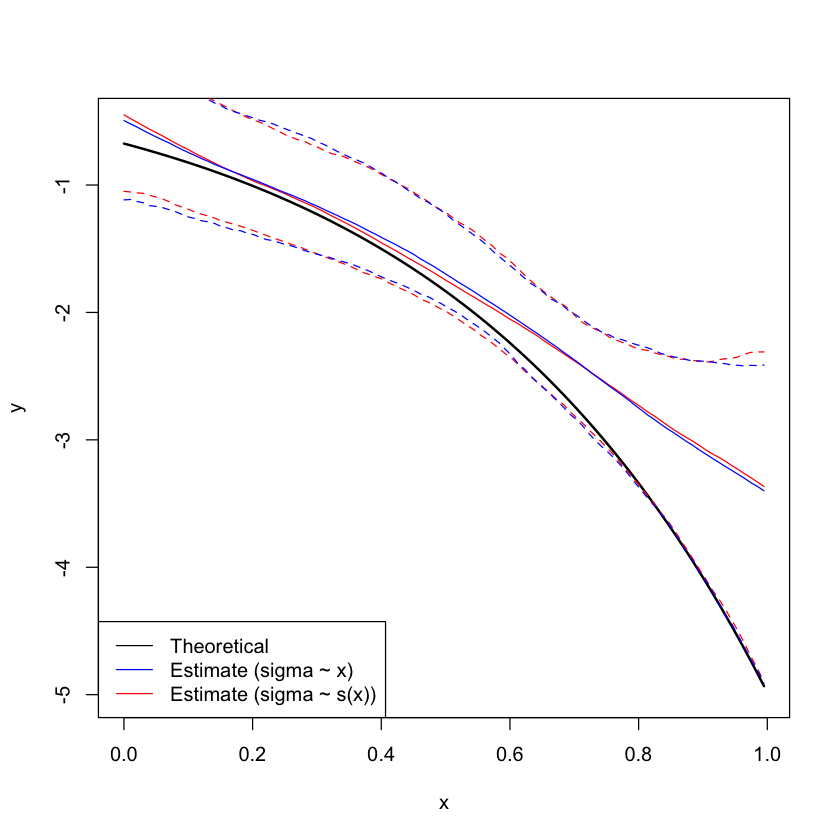
\includegraphics[width=.8\textwidth]{output.png}
    \caption{.25 quantile regression}
    \label{fig:output}
\end{figure}

Figure \ref{fig:output} shows the results. The estimates with both specifications are very similar.
And the theoretical quantile is within the 95\% credible interval.

The next thing we tried was using non-centered data. We used data with linearly and quadratically growing means. 
Figure \ref{fig:output2} shows one instance of the results. 
Again, the theoretical quantile is within the 95\% credible interval.

\begin{figure}[ht]
    \centering
    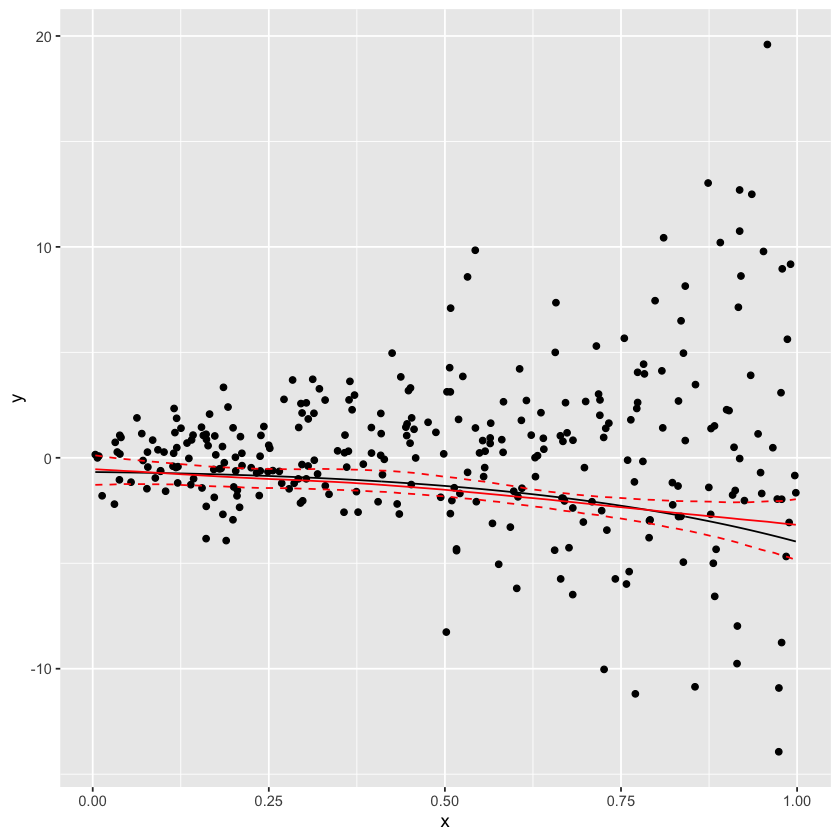
\includegraphics[width=.8\textwidth]{output2.png}
    \caption{.25 quantile regression on non centered data}
    \label{fig:output2}
\end{figure}

\section{Bayesian SEM}

Last week, we started exploring using BRMS to do handle latent variables. 
Let me ellaborate on that. 
The model we have in mind has a couple of latent variables.
One of them depends linearly on some covariates and is measured with error. 
The other one depends on the first and on the covariates through smooth functions. 
The output of the model are a set of observed variables that are regressions of the second latent variable. 

This week, we first implemented a simulation of that model. 
Second, we tried fitting it with Bayesian methods. 
Specifically, we tried using both BRMS and \lstinline{blavaan}. 

The results of this second step were mixed. 
We started by simplifying the assumptions, taking the smooth functions mentioned above to be linear.
Even in that case, BRMS was not at all able to handle the added complexity of the model. 
Lots of divergences were generated and the estimates were completely off.
On the other hand, \lstinline{blavaan} produced a good fit.
However, \lstinline{blavaan} has a serious limitation: 
it does not couple nicely with splines or other non-parametric methods. 

During the coming week, we will try to impose restrictiong on the priors used by BRMS to see if that helps.



\end{document}